
\documentclass[conference]{IEEEtran}
\usepackage{color}

% *** MISC UTILITY PACKAGES ***
%
%\usepackage{ifpdf}
% Heiko Oberdiek's ifpdf.sty is very useful if you need conditional
% compilation based on whether the output is pdf or dvi.
% usage:
% \ifpdf
%   % pdf code
% \else
%   % dvi code
% \fi
% The latest version of ifpdf.sty can be obtained from:
% http://www.ctan.org/tex-archive/macros/latex/contrib/oberdiek/
% Also, note that IEEEtran.cls V1.7 and later provides a builtin
% \ifCLASSINFOpdf conditional that works the same way.
% When switching from latex to pdflatex and vice-versa, the compiler may
% have to be run twice to clear warning/error messages.

\usepackage{cite}
% cite.sty was written by Donald Arseneau
% V1.6 and later of IEEEtran pre-defines the format of the cite.sty package
% \cite{} output to follow that of IEEE. Loading the cite package will
% result in citation numbers being automatically sorted and properly
% "compressed/ranged". e.g., [1], [9], [2], [7], [5], [6] without using
% cite.sty will become [1], [2], [5]--[7], [9] using cite.sty. cite.sty's
% \cite will automatically add leading space, if needed. Use cite.sty's
% noadjust option (cite.sty V3.8 and later) if you want to turn this off.
% cite.sty is already installed on most LaTeX systems. Be sure and use
% version 4.0 (2003-05-27) and later if using hyperref.sty. cite.sty does
% not currently provide for hyperlinked citations.
% The latest version can be obtained at:
% http://www.ctan.org/tex-archive/macros/latex/contrib/cite/
% The documentation is contained in the cite.sty file itself.

\usepackage{hyperref}


% *** GRAPHICS RELATED PACKAGES ***
%
\ifCLASSINFOpdf
  \usepackage[pdftex]{graphicx}
  % declare the path(s) where your graphic files are
  % \graphicspath{{../pdf/}{../jpeg/}}
  % and their extensions so you won't have to specify these with
  % every instance of \includegraphics
  \DeclareGraphicsExtensions{.pdf,.jpeg,.png}
\else
  % or other class option (dvipsone, dvipdf, if not using dvips). graphicx
  % will default to the driver specified in the system graphics.cfg if no
  % driver is specified.
  % \usepackage[dvips]{graphicx}
  % declare the path(s) where your graphic files are
  % \graphicspath{{../eps/}}
  % and their extensions so you won't have to specify these with
  % every instance of \includegraphics
  % \DeclareGraphicsExtensions{.eps}
\fi
% graphicx was written by David Carlisle and Sebastian Rahtz. It is
% required if you want graphics, photos, etc. graphicx.sty is already
% installed on most LaTeX systems. The latest version and documentation can
% be obtained at:
% http://www.ctan.org/tex-archive/macros/latex/required/graphics/
% Another good source of documentation is "Using Imported Graphics in
% LaTeX2e" by Keith Reckdahl which can be found as epslatex.ps or
% epslatex.pdf at: http://www.ctan.org/tex-archive/info/
%
% latex, and pdflatex in dvi mode, support graphics in encapsulated
% postscript (.eps) format. pdflatex in pdf mode supports graphics
% in .pdf, .jpeg, .png and .mps (metapost) formats. Users should ensure
% that all non-photo figures use a vector format (.eps, .pdf, .mps) and
% not a bitmapped formats (.jpeg, .png). IEEE frowns on bitmapped formats
% which can result in "jaggedy"/blurry rendering of lines and letters as
% well as large increases in file sizes.
%
% You can find documentation about the pdfTeX application at:
% http://www.tug.org/applications/pdftex





% *** MATH PACKAGES ***
%
\usepackage[cmex10]{amsmath}
% A popular package from the American Mathematical Society that provides
% many useful and powerful commands for dealing with mathematics. If using
% it, be sure to load this package with the cmex10 option to ensure that
% only type 1 fonts will utilized at all point sizes. Without this option,
% it is possible that some math symbols, particularly those within
% footnotes, will be rendered in bitmap form which will result in a
% document that can not be IEEE Xplore compliant!
%
% Also, note that the amsmath package sets \interdisplaylinepenalty to 10000
% thus preventing page breaks from occurring within multiline equations. Use:
\interdisplaylinepenalty=2500
% after loading amsmath to restore such page breaks as IEEEtran.cls normally
% does. amsmath.sty is already installed on most LaTeX systems. The latest
% version and documentation can be obtained at:
% http://www.ctan.org/tex-archive/macros/latex/required/amslatex/math/

\usepackage[font=footnotesize,labelsep=period]{caption}
\renewcommand{\figurename}{Figure}
%\usepackage[font=footnotesize]{subfig}
% subfig.sty, also written by Steven Douglas Cochran, is the modern
% replacement for subfigure.sty. However, subfig.sty requires and
% automatically loads Axel Sommerfeldt's caption.sty which will override
% IEEEtran.cls handling of captions and this will result in nonIEEE style
% figure/table captions. To prevent this problem, be sure and preload
% caption.sty with its "caption=false" package option. This is will preserve
% IEEEtran.cls handing of captions. Version 1.3 (2005/06/28) and later
% (recommended due to many improvements over 1.2) of subfig.sty supports
% the caption=false option directly:
%\usepackage[caption=false,font=footnotesize]{subfig}
%
% The latest version and documentation can be obtained at:
% http://www.ctan.org/tex-archive/macros/latex/contrib/subfig/
% The latest version and documentation of caption.sty can be obtained at:
% http://www.ctan.org/tex-archive/macros/latex/contrib/caption/

\usepackage{fixltx2e}
\usepackage{stfloats}

%\usepackage{url}


% correct bad hyphenation here
\hyphenation{op-tical net-works semi-conduc-tor}

\usepackage{xcolor}
\usepackage{flushend}
%\usepackage{fancyvrb}
\usepackage{listings}
\lstset{%
basicstyle=\small\ttfamily,
keywords=\bfseries,
showstringspaces=false,
identifierstyle=,
escapeinside={||},
mathescape=true,
morekeywords={TABLE,FOR,AS,READONLY,FIELDS,MAPFD,MAPLNKTBL,MAPKIND,VIEW},
morestring=[b]',
stringstyle=\ttfamily,
}

\colorlet{pcolor}{blue}
\colorlet{fcolor}{red}
\newcommand{\e}[2][fcolor]{\textcolor{pcolor}{[}\textcolor{#1}{#2}\textcolor{pcolor}{]}}

\hypersetup{
    bookmarks=true,         % show bookmarks bar?
    unicode=true,           % non-Latin characters in Acrobat’s bookmarks
    pdftoolbar=true,        % show Acrobat’s toolbar?
    pdfmenubar=true,        % show Acrobat’s menu?
    pdffitwindow=false,     % window fit to page when opened
    pdfstartview={FitH},    % fits the width of the page to the window
    pdftitle={A Semantic Markup Technique Based on Ontology Polysystem},    % title
    pdfauthor={Evgeny Cherkashin, Kristina Paskal, Igor Bychkov},     % author
    pdfsubject={Scientific paper},   % subject of the document
    pdfcreator={LaTeX},   % creator of the document
    pdfproducer={LaTeX}, % producer of the document
    pdfkeywords={polysystem} {ontology} {semantic web} {knowledge
      acquisition} {data mining} {natural language processing}, % list of keywords
    pdfnewwindow=true,      % links in new window
    colorlinks=true,       % false: boxed links; true: colored links
    %linkcolor=[rgb]{0 0.4 0.1},          % color of internal links (black)
    linkcolor=black,          % color of internal links (black)
    %citecolor=blue,        % color of links to bibliography
    citecolor=black,        % color of links to bibliography
    filecolor=black,      % color of file links
    %urlcolor=[rgb]{0.3 0.0 0.3}           % color of external links
    urlcolor=black           % color of external links
}

\newenvironment{asdcode}{\hangindent=\parindent\hangafter=1\par\noindent\small\tt}{}


\begin{document}
\title{A Descriptive Specification Tools for Information System Design and Configuration}
  \author{%
   \IEEEauthorblockN{%
    Alexey Hmelnov\IEEEauthorrefmark{1}\IEEEauthorrefmark{2},
    Evgeny Fereferov\IEEEauthorrefmark{1},
    Roman Fedorov\IEEEauthorrefmark{1}\IEEEauthorrefmark{2},
    Evgeny Cherkashin\IEEEauthorrefmark{1}\IEEEauthorrefmark{2}\IEEEauthorrefmark{3} %, \\
%    Polina Belykh\IEEEauthorrefmark{1},
%    Alexander Zamashikov\IEEEauthorrefmark{3}
   }%
  \IEEEauthorblockA{\IEEEauthorrefmark{1}Institute of System Dynamics
    and Control Theory at SB RAS, Irkutsk, Lermontov str., 134,
    664033, Russia}%
  \IEEEauthorblockA{\IEEEauthorrefmark{2}Irkutsk State University,
    Irkutsk, Gagarina blvd., 664003, Russia}%
  \IEEEauthorblockA{\IEEEauthorrefmark{3}National Research Irkutsk
    State Technical University, Irkutsk, Lermontov str., 83, 664074,
    Russia}%
\texttt{\small \{alex,fereferov,fedorov,eugeneai\}@icc.ru}
}

% use for special paper notices
%\IEEEspecialpapernotice{(Invited Paper)}

% make the title area
\maketitle

\def\thepage{Page \arabic{page}}
%\setcounter{page}{252}

\begin{abstract}
Software development technologies evolved from concrete algorithm design and their programmatic implementation to modeling the whole information systems (IS).  The modeling approaches allows developers to describe the system in terms of domain, software design, properties of implementation platforms, and standard ways of the IS development such as programming traditions in a concrete firm.  In the case if a new IS is being constructed, having an already implemented database, Data Driven Engineering (DDE) is used.  The model of this IS is constructed by importing database structure and adding a semantic layer description reflecting the database structure to the domain terms.

We describe a DDE-approach based on declarative specifications of existing database schema and properties of the target application, as well as interpretation of the description into IS components.  The interpretation in various aspects allows developer to construct user interface for database modification, subsystem of SQL query construction in terms of domain, etc.  An example result is presented.

%The obtained description could be used to extend the capabilities of SQL query constructor to allow user formulating the query in a natural language, e.g. in Russian.  In order to do so a new layer of the domain and IS properties description should be devised.  The layer is based on an ontological description of the domain referencing the terms of the database description.  The layer also is to be reflected to morphological structures of the natural language used to formulate the queries.
\end{abstract}


% For peer review papers, you can put extra information on the cover
% page as needed:
% \ifCLASSOPTIONpeerreview
% \begin{center} \bfseries EDICS Category: 3-BBND \end{center}
% \fi
%
% For peerreview papers, this IEEEtran command inserts a page break and
% creates the second title. It will be ignored for other modes.
\IEEEpeerreviewmaketitle



\section{Introduction}
% no \IEEEPARstart
Software development technologies evolved from concrete algorithm design and their programmatic implementation to modeling the whole information systems (IS).  The modeling approaches allows developers to describe the system in terms of domain, engineering and software design, features of implementation platforms and tools, and standards of the IS development of a software firm such as programming traditions, used modeling and instrumental tools, etc.  This extends nowadays production developer philosophies referred to as DRY (Do not Repeat Yourself), where each concept in a system must be defined only once.  DRY is a basis of many open-source web development frameworks such as Django [].

The theoretical basis of the modeling approach is model transformation theories and their software implementations, which are developed in the field of Model Driven Engineering (MDE).  The transformations construct ultimately either source code modules realizing modeled structures or an operator interpretation of models of an intermediate level like virtual machine byte code, SQL queries execution plan synthesis, and executable UML.  Model transformation is based on recognition of a pattern structures in the source model, relating them to the model of development platform rules of transformation.  The results of transformation are  structures of a model of more specific (concrete) level of abstraction.  At the lowest level the code generation routines are executed, which use source code templates.  Thus, from the point of view of generative programming, one of main function of the transformation process is an intelligent configuration generation for the source code generators.

In the case if new IS is being constructed, having already designed and deployed database, Data Driven Engineering (DDE, a kind of MDE) is used.  The model of this IS is constructed by importing database structure, e.g. DDL-queries, analyzing it, and adding a semantic layer of the database structure description in IS's domain concepts and relations.  In Laboratory of Complex Information Systems of Institute of System Dynamics and Control Theory at Siberian Branch of Russian Academy of Sciences, a number of DDE approaches has been developed based on declarative specifications and their run time interpretations, as well as techniques automating the description process.  The interpretation in various aspects allows developer to construct user interfaces for database modification, subsystem of SQL-queries construction in terms of domain, plugin integration, etc.

The report describes an DDE-approach of IS development based on a special specification language describing database properties, interpretation of the description in various IS components, resulting in automatic user interface construction and layouting, constraint-oriented database editor, SQL-query builder, OLAP subsystem, etc.

\section{The Description Language}
\label{sec:description-database}

%Data Driven Engineering (DDE) \cite{DDE} one of the powerful direction of Computer science allowing to construct software on the base of data models (data structure description).  Being a part of Model Driven Engineering, DDE inherits its main thesis that software development is a sequence of model transformations starting from abstract models describing information system (IS) in terms of domain \e{and software development process}.

The DDE-modeling of an IS starts either from description of a general view of data structures used by business-logic or from loading schema of already existing database.  The second case has important value in practice, when customer requires a new implementation of an exiting IS with new features and with conserving exiting data in its warehouse.

The structural description allows developers implementing routine functionality via transformation and generation, e.g., data input forms; user interface and business-logic interaction; import, export and integration operations; etc.  Adding a domain description allows one to refine user interface with notions familiar to user, as well as construct various query-answering subsystems like SQL-query builders and OLAP operating in terms of domain.

In Institute of System Dynamics and Control Theory at SB RAS a number of DDE technologies has been developed within economic contracts activities supported by necessary theoretical investigations.  One of the last description format is based on mix of the \texttt{.ini}-file and SQL-query languages.  The first format is used to describe database structure and semantic of attributes and their relations, the second part is used to describe the rules of user interface generation, and interaction with geographical information systems and other applications.

\subsection{Development Stages}
\label{sec:descr-synth-stag}

In the proposed approach, in a general case on the first stage of IS development, system engineer carries on structural analysts of the domain, resulting in description of concepts and their basic relations, business-processes and software requirements.  After that, at the second stage, the database design follows, which produces database schema ad its implementation as database server.  Common design tools (such as Sybase Power Designer, IBM Rational Rose) are used on this stage.

On the third stage, model of IS is constructed by loading the implemented database schema and extending it with the description of the following special database object classes: \texttt{TABLE}, \texttt{VIEW}, \texttt{RULE}, and so called \emph{superstructure}.  The \texttt{TABLE} objects describe IS database structure and relations, attribute data types and names.  These object are automatically constructed by loading and analyzing IS database schema, if it is literally devised (it must be at least in third normal form).  The lack of schemata data is compensated manually with the description language and the following interpretation.

The \texttt{VIEW} objects are more complicated than \texttt{TABLE} ones, which is used to generate user interface.  Here we define properties of the attribute and table relations, for example, for each foreign key a look-up widget can be used to select a record from a foreign table (a reference book).  For complex reference book and transitive references, the key attribute sets bust be specified to increase generated user interface usability.  There are other special cases of foreign key interpretations, like ``master-details'', and all of them can be specified with the specification language.

The \emph{superstructure} objects support interaction of developed IS with foreign modules and libraries, processing information with methods beyond the standard of rational databases and SQL, e.g., computer simulation and complex data visualizations.

%\hangindent=\parindent%\hangafter=1
The \texttt{RULE} objects are responsible for expression of functions implementation in generated IS specific to its business-processes.  By means of the rules, one can describe input field logic (enabling and disabling them), implement uniqueness check routines and plug-in modules interaction, i.e., rules provide declarative means of describing and implementing relationships between objects and components in business-logic layer of IS.  The rules also affect the generated queries to IS database during editing, as well as creating special widgets in user interfaces, which connect input data with spatial tables and render cartographic. For all the object classes a formal set model is devised [] and investigated.  %We will not describe it in this paper, ...}

On the forth stage the IS functionality is generated at run time as a result of the specification interpretations.  It integrates foreign software subsystems according to the rules. %\e[blue]{Should we describe the rules of interface generation in details ?}

\subsection{The Description Language}

Our specification language is reasonably simple whereas complete with respect to expressive ability.  The language has LL(1) grammar class.  Its syntactic structures describe elements of IS and a general options like database connection properties.  The specifications written in the language are \emph{precise}, \emph{understandable} and \emph{complete} according to [1,2].  The language clauses have the following general structure:

\begin{asdcode}%
<Start keyword> <List of mandatory statements> [~list of optional statements~]
\end{asdcode}

The \texttt{Start keyword} can be one of the following: \texttt{ADO}, \texttt{BDE}, \texttt{CFG}, \texttt{TABLE}, \texttt{VIEW}, \texttt{PLUGINS}, \texttt{USES}, \texttt{INCLUDE}, \texttt{MENU}.  First two are used to describe properties of database connection.  Keyword \texttt{CFG} used to describe general application settings of IS.  Keywords \texttt{TABLE}, \texttt{VIEW} describe the database schema and view widgets.  Keyword \texttt{PLUGINS} describes interaction with outer systems; \texttt{USES} and \texttt{INCLUDE} allow developer to break an IS description into source modules.  Keyword \texttt{MENU} controls the main menu of IS application.

Let's consider a part of an example description.

\begin{lstlisting}
TABLE ADR FOR SP_ADDR AS 'Address' READONLY
\end{lstlisting}

This statement describes table \texttt{SP\_ADR} of IS, the table will have an alias \texttt{ADR} for usage in the rest of the specification.  The table will have also a user-friendly alias \texttt{'Address'} in user interface forms, table editor, etc.  The following language construction describes table fields.

\begin{lstlisting}
FIELDS (ID_BUIL_G P AS 'Building Code',
        ID_NREG ^SP_NREG AS 'Region Code',
 ID_MK_GM ^SP_MK_GM AS 'Microdistrict Code',
        ID_STREET ^vSP_STR AS 'Street Code',
        BUIL=S AS 'Building',
        ANN=S AS 'Annotation);
\end{lstlisting}%

Identifiers \texttt{ID\_*}, \texttt{BUIL} and \texttt{ANN} are table fields.  Sign \texttt{\^} creates a reference to a table or a view, in particular, \texttt{\^{}SP\_NREG} is a table referenced by field \texttt{ID\_NREG}, and \texttt{\^{}vSP\_STR} is a reference to a view.  Expression \texttt{ANN=S} denotes that \texttt{ANN} is a string field.  At the first line of the example, \texttt{ID\_BUIL P} denotes that the field is a key field.

There are also more sophisticated ways of various reference denotation, expressed with a general \texttt{REFS(\ldots)} construction.  Its parameters that allows one to define references of various IS business-logic interpretations including ``master-details'', special cases of ``reference book'' and so on.

\section{Interpretations of the Description}
\label{sec:interpr-descr}

All current implementations of the interpretation of the specification language are run time.  After preparing the specification of the IS database, the IS developer must run the IS environment with the specification an the database as its input.  The specification is translated, and the translator creates two data structures.  One is stored in process memory as complex data structures and used by form and query builders.  Another one is a technical database of tables, describing IS database structures.  The technical database is used by database editor and OLAP modules.  The translator also check whether the specification is changed and corrects the database accordingly.

\subsection{User Interface Generation}
\label{sec:user-interace-form}
One of the important IS quality characteristics is its input forms, and layouting the widgets in the forms is the question of usability.  From one hand side the widgets must efficiently consume the area of a form, and on another hand side, the user interface must be convenient and fit to  application functionality requirements.

The change of form size results in relayouting the widgets if the form is aware of the change.  Various software development environments support the problem solution differently.  E.g., an Embarcadero Delphi developer must specify \texttt{align}, \texttt{anchors} and \texttt{autosize} properties of a widget to adjust the widgets behavior upon form size change.  The operation must be performed for each widget, and in conditions of entering of a database record of many attributes the adjustment process is routine and time consuming.  In addition, layout mechanics of Delphi cannot distribute the size variations among widgets proportionally.

The problem is partially solved in, e.g., open-source widget libraries, like Qt and GTK+ [,].  The widgets are placed in so called containers (which are also a virtual widgets), which manage thir order, spacing, padding, fill and expansion properties.  GTK+ widgets could also issue special size request message to notify parent widget about required minimal size.  Nevertheless the general engines implemented in the instrumental systems are not aware of the attribute data properties of the IS database.

To account the domain properties of attributes, a rule-based engine has been developed on the base of the database specification.  The engine interprets the database specification, adjusts Database Editor widget, and generates form for database records modification.

\paragraph{Database Editor}

Database Editor controls a dynamic user interface operating over IS database records.  Its layout includes three areas (panels): menu of entities, operations, and data table itself.  Menu of entities (fig.~\ref{fig:dbeditor}, left panel) consist of database and view table names described in the specification.  The entities are joined in semantic groups according to their roles and functions.

\begin{figure}[tb]
  \centering
  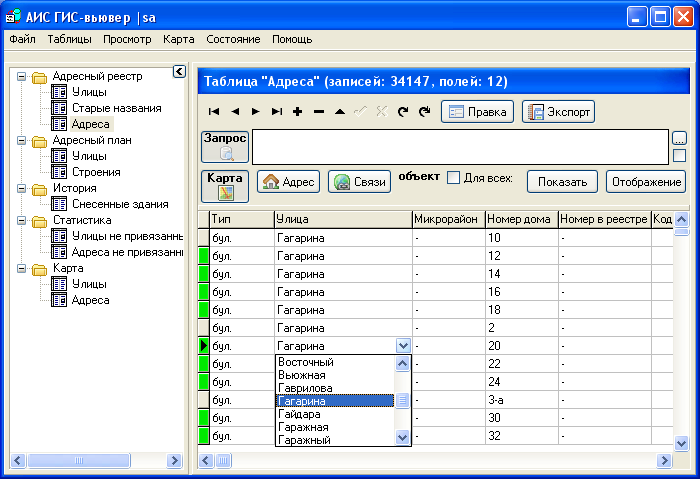
\includegraphics[width=\linewidth]{dbeditor.png}
  \caption{Database editor}
  \label{fig:dbeditor}
\end{figure}

The operation area (fig.~\ref{fig:dbeditor}, top panel) displays widgets for construction and execution of data processing operations.  The set of widgets for each table (view) is controlled by the specification.  The minimal set contains table navigation buttons, ``Edit'', ``Export'' and ``Query'' buttons.  Optional buttons are ``Options'' and ``Cartographic''.  The layout of the widgets in under control of layout manager.

The table area (fig.~\ref{fig:dbeditor}, bottom-right panel) displays chosen entity.  The data is represented in two views: tabular and as a form.  Tabular form supports standard data editing operations, but they adjusted according to specification: reference fields are choice boxes and look-up widgets.  Dependable (in sense of the specification) fields are changed as soon as their ascendant become edited.  For example, in fig.~\ref{fig:dbeditor} street name in an address record is chosen from a look-up list of streets.  The street \texttt{ID} is stored in an address reference field, this results in changing address \texttt{TYPE} (boulevard or street) field according to the type of chosen street.

The order and widths of the table columns can be adjusted according to user's preferences.  The customization is stored in user profile \texttt{.wsf}--file.

\paragraph{Form Mode}

Form mode is a generated user interface for table record editing with accounting table's references to other tables, views and visual components.  The form mode is activated from Database Editor with mouse click, button ``Edit'' and creation of new record.  The layout of the widgets of the form is generated according to the database specification and run time context: whether this record belongs to a main table or a reference one.  Each attribute editing widget is accompanied with a label showing user-friendly attribute alias from the specification.  The label can signify attributes uniqueness, non-null condition and a membership in the primary key.

For each widget, placement, order, widths and width adjustment are controlled by layout manager component.  The order and layout of the form must conform to criteria of usability.  Upon form size change or screen resolution the widgets must be reordered, resized, and so on, conversing the usability criteria \e{as much as possible}.  The layout manager extends ideas of FlowLayout [76] (Java): the widgets a placed in rows from left to right.  FlowLayout manager implies that each widget has fixed size.  We took over the restriction, and our layout manager takes advantage of some heuristics based on minimal (\texttt{szMin}), best (\texttt{szBes}), and maximal (\texttt{szMax}) sizes of a widget.  Maximal size is equal to field data size, e.g., for \texttt{VARCHAR(150)} field, the \texttt{szMax} is equal to 150.  Experience shows that it is more ergonomic to display about 70~\% of \texttt{szMax}, and it is \texttt{szBest}.  Minimal size for strings is taken about 10 characters.

The layout manager arranges the widgets according to the following strategy.  At the first stage all three sizes are queried from the widgets, and tries to figure out a layout, where all the widgets have maximal sizes and placed in rows from left to right.  If a widget is not shown in the form, the layouting immediately restarts the process, with \texttt{szBest} used as widgets sizes.  In the last case, if the layout process finished successfully and there are some free space, then the layout manager tries to extend significant widgets to their maximal sizes.  In the wort case, when the second try has failed, the manager uses \texttt{szMin}.

The developed ... (group boxes) . An example of auto.... foem ish sown in fig.~\ref{fig:formex}.

\begin{figure}[tb]
  \centering
  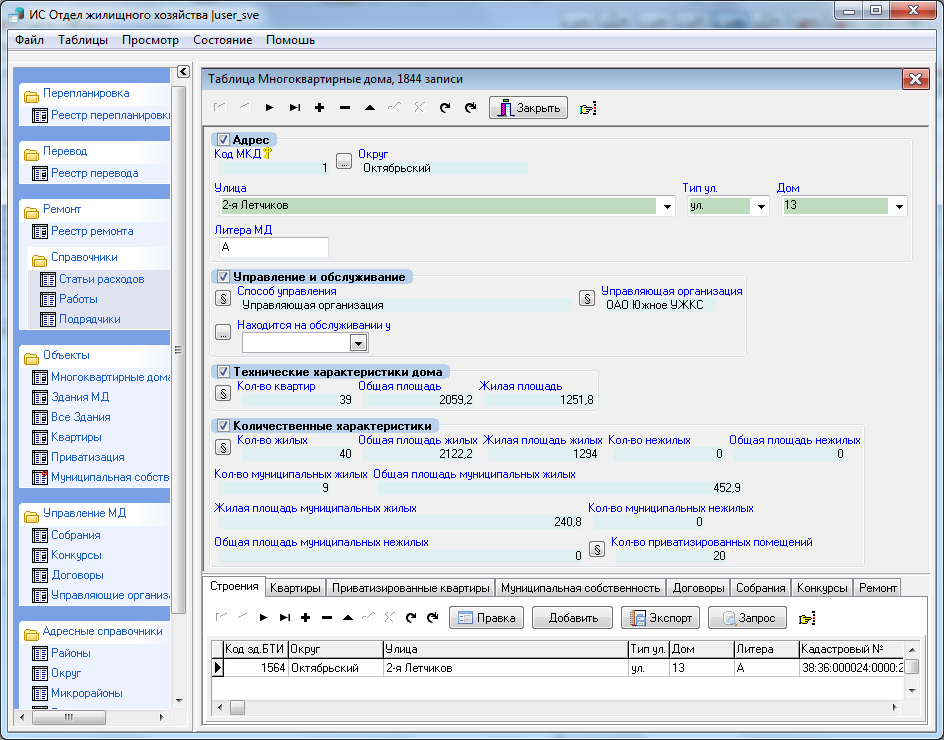
\includegraphics[width=\linewidth]{formex.png}
  \caption{An example of autolayout form}
  \label{fig:formex}
\end{figure}

\subsection{Query Builder}
\label{sec:query-builder}

Most of IS applications require components for data search and filtering.  An expressive user-friendly search engine allows one to quickly jump to a specific record and also allow subject specialist to query record data from database without programmers assistance.

Query constructor of Microsoft Access allows user to design a complex SQL-queries for aggregating and modifying data.  The query builder supports definition of complex conditions for the \texttt{WHERE} and \texttt{HAVING} sections of the query.  The query builder also does not account the domain, and, thus, it is intended for programmers and experienced users accounted with database technologies.  Another problem is the availability of the SQL-query designer utilities for web projects.

In our work we proposed an engine [62] that supports interactive specification of field value criteria and construction of combinations of logical and filter operations sufficient to describe common user queries.  Query builder is a form that is adjusted to a table according to the specification of IS database.  The logical condition is a tree structure, which is drawn horizontally to allow long field names to be displayed correctly without overlapping.

To control the tree editing, a special widget has been developed.  The widget placed inside a dialog windows is shown in fig.~\ref{fig:qbuilder}.  The widget allows to construct tree from elementary operations, move the operations between various levels of folding, operand switching, editing criteria values.

\begin{figure}[tb]
  \centering
  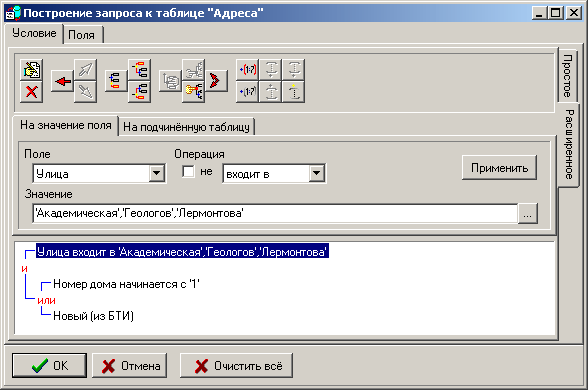
\includegraphics[width=\linewidth]{qbuilder.png}
  \caption{User controlled query builder}
  \label{fig:qbuilder}
\end{figure}


\subsection{On-Line Analitical Processing}
\label{sec:olap}

The IS description used to implement import routines for On-Line Analitical Processing unit (OLAPu).  The unit allows user to store, select and analyze numberic indicators.  The indicators are considered as funtions of a set of attributes.  OLAPu can
selected the indicators in various projection combinations.

OLAPu's design is classic client-server architecture, where server is a rational data storage, and client provide a flexible access to the indicator data by means of intuitive user interface.  The interface is configured specially to support the munidimentional OLAP.  The user by means of widgets of the interface selects and ajusts projection and indicator aggregation configuration, the results of the configuration are presented ast interactive tables and can be stored in Microdoft Excel spreadsheet pages.

To convert IS data {table}, {view} and {superstructure} objects are used.  The data converts into a tree of indicators.  Each node of tree correspond data selected in a projection.  Each projection characterizes with a set of attributes.  The sets are reffered as dimentions.  They could describe regions, industries, types of ownership, etc.  A special case of the dimentions is time intervals, such as year, half a year, quartal, month.  Most of the indicators are tied with time intervals.

The indicator data usually have more complex structure than just a linearly ordered set.  The set usually is a tree structure, where one inidcator aggregates data of a set of subordinal indicators, e.g., state indicator aggregates state regional data.  The same is true for industries.  The indicators are stored in indicator value tables.  The table includes all the index dimension attribute references to the tables of the IS database and the index value itself.

\begin{figure}[bt]
  \centering
  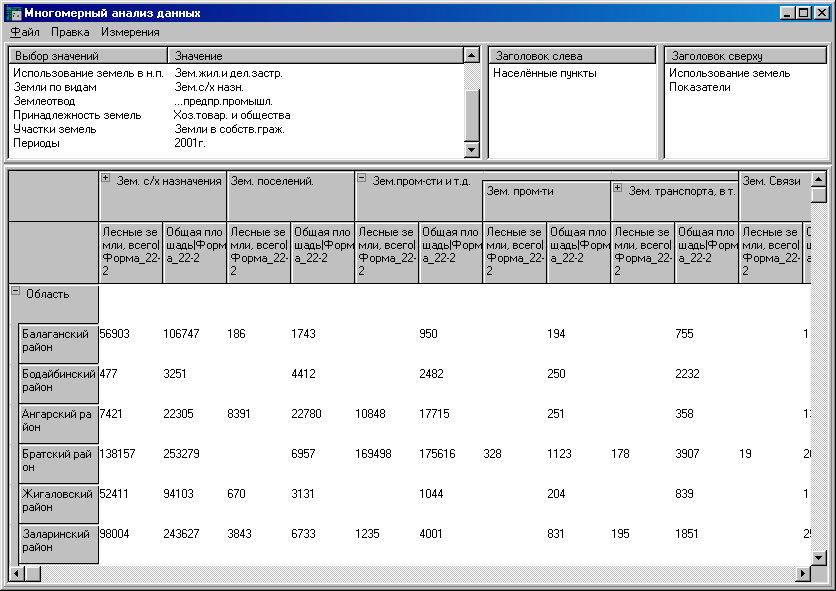
\includegraphics[width=\linewidth]{MDA-olap.png}
  \caption{Main window of OLAP unit}
  \label{fig:olapu}
\end{figure}

The main windows of OLAP unit is shown in fig.~\ref{fig:olapu}.  The window has been divided on two parts.  The upper part consist of three panels with dimension lists, and the lower part is the resulting table.  User must select an indicator from the left list of dimensions as well as the dimensions associated with columns and rows of the resulting table.  The headers of rows and columns may contain combinations of dimensions.  In this case for all the combination a row (column) is inserted into the resulting table widget.  The combinations of dimensions and attribute value filters are adjusted by mouse click on the tables.

The time intervals are selected with special pop up dialog widget on mouse click.  User can drag dimensions between lists and reorder them, this results in regeneration of the resulting table.  When editing is allowed, user can change values of indicators directly in the resulting table cells.  The changes are immediately stored into the original database of IS.  The table widget allows export data and table structure into system clipboard in a table format recognizable by Microsoft Excel, the same is implemented in the opposite direction.

\e[blue]{Import data. Needed?}


\section{GIS Integration: an Usage Example}
\label{sec:gis-integration}

The developed technologies are applied in GeoAW (Geological Automatized Workplace) environment, which is aimed at construction of GIS for municipal authorities.  Its derivative GIS systems allow one to represent data accumulated in departments as GIS cartographic.  In order to construct such system developers must go through the steps described early to describe data sources and filter data to be represented in new GIS applications.  The main attention should be paid to spatial related attributes, as the attributes are used in connecting the table rows and graphics shapes of topographic base.

GeoAW environment is an instrumental tool to create stand-alone Windows GIS applications.  Its architecture is shown in fig.~\ref{fig:architecture}.  GeoAW consists of the following main software components: Specification Management,  System Kernel, Database Editor, user Query Builder, Plugin Interface, and GIS as external application.
\begin{figure}[bt]
  \centering
  \def\svgwidth{\linewidth}
  \tiny\sffamily
  \def\db{Database}
  \def\spec{Specification}
  \def\sce{\vtop{Specification\break Management}}
  \def\kerne{Kernel}
  \def\bde{\vtop{Database\break Editor}}
  \def\qb{\vtop{Query\break Builder}}
  \def\map{GIS}
  \def\gb{Graphic Base}
  \def\plug{Plugins}
  \def\intfs{\vtop{Plugin\break Interface}}
  \input{GeoAWArch.pdf_tex}
  \caption{GeoAW instrumental environment architecture}
  \label{fig:architecture}
\end{figure}

\e{The GeoAW Delphi}

The following description is necessary part example of the whole model as it describes the root table \e[blue]{and its view}.

\begin{lstlisting}
VIEW vSP_ADR FOR ADR AS 'All Addresses'
|\textbf{NAMES}|='U;BUIL' |\textbf{ADDRS}| ='U;BUIL'
MAPFD=ID_BUIL_G MAPLNKTBL=MAP_LNK MAPKIND=1
FIELDS (ID_BUIL_G= AS 'Building Code',
        [GB='Address',
         R=ID_NREG.REGION AS 'Region',
         M=ID_MK_GM.MK_GM AS 'Microdistrict',
         T=ID_STREET.STREET_TYPE AS 'Type',
         U=ID_STREET.STREET AS 'Street',
         BUIL= AS 'Builfing']
        [DGB='Buildongs at Address'],
         ANN= AS 'Annotation');
\end{lstlisting}

\begin{figure}[tb]
  \centering
  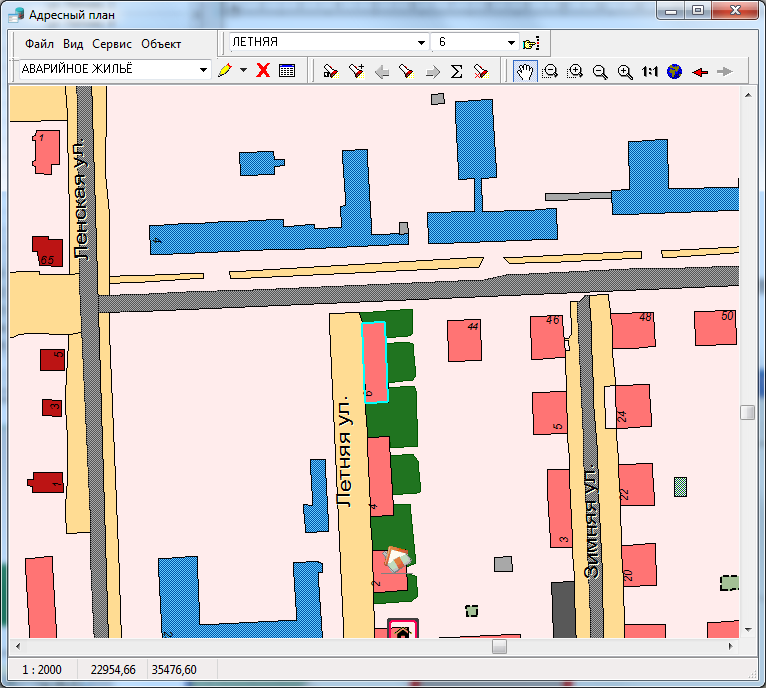
\includegraphics[width=\linewidth]{addressplan.png}
  \caption{Address plan GIS window}
  \label{fig:addrplan}
\end{figure}


% An example of a floating figure using the graphicx package.
% Note that \label must occur AFTER (or within) \caption.
% For figures, \caption should occur after the \includegraphics.
% Note that IEEEtran v1.7 and later has special internal code that
% is designed to preserve the operation of \label within \caption
% even when the captionsoff option is in effect. However, because
% of issues like this, it may be the safest practice to put all your
% \label just after \caption rather than within \caption{}.
%
% Reminder: the "draftcls" or "draftclsnofoot", not "draft", class
% option should be used if it is desired that the figures are to be
% displayed while in draft mode.
%

% Note that IEEE typically puts floats only at the top, even when this
% results in a large percentage of a column being occupied by floats.


% An example of a double column floating figure using two subfigures.
% (The subfig.sty package must be loaded for this to work.)
% The subfigure \label commands are set within each subfloat command, the
% \label for the overall figure must come after \caption.
% \hfil must be used as a separator to get equal spacing.
% The subfigure.sty package works much the same way, except \subfigure is
% used instead of \subfloat.
%
%\begin{figure*}[!t]
%\centerline{\subfloat[Case I]\includegraphics[width=2.5in]{subfigcase1}%
%\label{fig_first_case}}
%\hfil
%\subfloat[Case II]{\includegraphics[width=2.5in]{subfigcase2}%
%\label{fig_second_case}}}
%\caption{Simulation results}
%\label{fig_sim}
%\end{figure*}
%
% Note that often IEEE papers with subfigures do not employ subfigure
% captions (using the optional argument to \subfloat), but instead will
% reference/describe all of them (a), (b), etc., within the main caption.


% An example of a floating table. Note that, for IEEE style tables, the
% \caption command should come BEFORE the table. Table text will default to
% \footnotesize as IEEE normally uses this smaller font for tables.
% The \label must come after \caption as always.
%
%\begin{table}[!t]
%% increase table row spacing, adjust to taste
%\renewcommand{\arraystretch}{1.3}
% if using array.sty, it might be a good idea to tweak the value of
% \extrarowheight as needed to properly center the text within the cells
%\caption{An Example of a Table}
%\label{table_example}
%\centering
%% Some packages, such as MDW tools, offer better commands for making tables
%% than the plain LaTeX2e tabular which is used here.
%\begin{tabular}{|c||c|}
%\hline
%One & Two\\
%\hline
%Three & Four\\
%\hline
%\end{tabular}
%\end{table}


% Note that IEEE does not put floats in the very first column - or typically
% anywhere on the first page for that matter. Also, in-text middle ("here")
% positioning is not used. Most IEEE journals/conferences use top floats
% exclusively. Note that, LaTeX2e, unlike IEEE journals/conferences, places
% footnotes above bottom floats. This can be corrected via the \fnbelowfloat
% command of the stfloats package.


\section{Conclusion}

The nowadays techniques of application software development are aimed at close cooperation of developer and customer.  To shift some responsibility to the customer's users and to extend the maintainability and usability of software, it is necessary to develop a techniques, which produce some processing according to a domain description.  ...

\e[blue]{Say, that form generator and database editor usually generates more usable forms that used before...}

In further work the obtained description could be used to extend the capabilities of SQL-query constructor to allow user formulating the query in a natural language in terms of modeled domain.  In order to do so a new layer of the domain and IS properties description should be devised.  The layer expands the description of the database entities and their relationships with abstract notions of domain and relations, resulting in fibered representation of the domain of two fibers: abstract domain and database structure.  The notions and relations are mapped through the fibers via interpretation.  \e{The layer is based on an ontological description of the domain referencing the terms of the database description.  The layer also is to be reflected to morphological structures of the natural language used to formulate the queries.}

\e{In this paper, we continue the development of the approach
\cite{fereferovDiss} within the theoretical aspect \cite{b2:15} of software unified model development, and briefly consider the approach of unification of software modeling and natural language processing.}

\e{Another direction is to... [Danil's Publication MIPRO'13]}


% conference papers do not normally have an appendix

% use section* for acknowledgement
\section*{Acknowledgment}
The research is carried on under support of Integration multidisciplinary project of Siberian Branch of Russian Academy of Sciences N 17 “Development of services and infrastructure of scientific spatial data for supporting complex multidisciplinary scientific research of Baikal nature territory”.

%The authors would like to thank...

% trigger a \newpage just before the given reference
% number - used to balance the columns on the last page
% adjust value as needed - may need to be readjusted if
% the document is modified later
%\IEEEtriggeratref{8}
% The "triggered" command can be changed if desired:
%\IEEEtriggercmd{\enlargethispage{-5in}}

% references section

% can use a bibliography generated by BibTeX as a .bbl file
% BibTeX documentation can be easily obtained at:
% http://www.ctan.org/tex-archive/biblio/bibtex/contrib/doc/
% The IEEEtran BibTeX style support page is at:
% http://www.michaelshell.org/tex/ieeetran/bibtex/
%\bibliographystyle{IEEEtran}
% argument is your BibTeX string definitions and bibliography database(s)
%\bibliography{IEEEabrv,../bib/paper}
%
% <OR> manually copy in the resultant .bbl file
% set second argument of \begin to the number of references
% (used to reserve space for the reference number labels box)
\urlstyle{tt}
\vspace{1.4em} % For no reason the reference was sticked to the
               % previous paragraph
\begin{thebibliography}{11}
\bibitem{TBL2001} T.~Berners-Lee, J.~Hendler, O.~Lissila. ``The
  Semantic Web A new form of Web content that is meaningful to
  computers will unleash a revolution of new possibilities,''
  Scientific American, May 17, 2001,
  pp.~1-18. URL:~\url{http://sciam.com/article.cfm?articleID=00048144-10D2-1C70-84A9809EC588EF21}
\bibitem{father} A.~K.~Cherkashin. ``Polysystem Analysis and
  Synthesis. Application in Geography,'' Novosibirsk, Russia ``Nauka'' Publ. co.
  1997. -- 502~p. (In Russian)
\bibitem{SN} Social network -- Wikipedia, the free encyclopedia.
  URL:~\url{http://en.wikipedia.org/wiki/Social_network} (access date: 09.01.2015).
\bibitem{prevwork} E.~Cherkashin, P.~Belykh, D.~Annenkov, K.~Paskal, ``A
  Document Content Logical Layer Induction on the Base of Ontologies
  and Processing Changes,'' Procs. of International Conference on
  Applied Internet and Information Technologies, October 25, 2013,
  University of Novi Sad, Technical Faculty ``Mihajlo Pupin'',
  Zrenjanin, Republic of Serbia,
  pp.~252--257. URL:~\url{http://www.tfzr.uns.ac.rs/aiit/archives/AIIT2013/Proceedings.pdf}.
\bibitem{b2:15} E.~Cherkashin, V.~Paramonov, et al, ``Model Driven
  Architecture is a Complex System,'' E-Society Journal Research and
  Applications. Volume 2, Number 2, 2011, pp.~15--23.
  URL:~\url{http://www.tfzr.uns.ac.rs/esociety/issues/eSocietyVol2No2.pdf} (access date: 09.01.2015).
\bibitem{b2:5} Model--view--controller --- Wikipedia, the free
  encyclopedia.
  URL:~\url{http://en.wikipedia.org/wiki/Model-view-controller} (access date: 09.01.2015.)
\bibitem{diff} D.~MacKenzie, P.~Eggert, R.~Stallman. ``Comparing and Merging Files,''
  URL:~\url{http://www.gnu.org/software/diffutils/manual/diffutils.pdf} (access date: 09.01.2015).
\bibitem{dectrees} Information gain in decision trees ---  Wikipedia, the free
  encyclopedia. URL:~\url{http://en.wikipedia.org/wiki/Information_gain_in_decision_trees}
\bibitem{zopetal} ``Zope Page Templates Reference,'' The Zope2 Book. URL:~\url{http://docs.zope.org/zope2/zope2book/index.html} (access date: 09.01.2015).
\bibitem{cham} Chameleon -- Chameleon 2.10 documentation.
  URL:~\url{http://chameleon.readthedocs.org/en/latest/}  (access date: 09.01.2015).
\bibitem{kiyoto} Kyoto Cabinet. URL:~\url{http://fallabs.com/kyotocabinet/} (access date: 09.01.2015).
\bibitem{mediawiki}
 Semantic MediaWiki. URL: \url{http://semantic-mediawiki.org/} (access date: 20.08.2013).
\bibitem{heino}
 N.Heino, S.Tramp, N.Heino, S.Auer. Managing Web Content using Linked Data Principles – Combining semantic structure with dynamic content syndication. Computer Software and Applications Conference (COMPSAC), 2011 IEEE 35th Annual. pp. 245 - 250. URL:\url{http://svn.aksw.org/papers/2011/COMPSAC_lod2.eu/public.pdf} (access date: 30.05.2013).

\end{thebibliography}
\vspace{-2em}\mbox{} %Make the flushend work correctly with the last \bibitem
% that's all folks
\end{document}

%%% Local Variables:
%%% mode: latex
%%% TeX-master: t
%%% End:
